\chapter{Análise de resultados}

Nesse capítulo, serão apresentados os dados, obtidos através da simulação, e realizada uma análise para avaliar as diferentes configurações utilizadas e seus impactos na fluxo do tráfego em um cruzamento. Os parâmetros adquiridos das simulações foram a duração da viagem de cada veículo em cada caminho (do ponto de partida até o ponto de chegada) e o tempo de espera em fila de cada caminho. Esses dados são adquiridos a cada passo da simulação, e utiliza os dados de todos os veículos que passam por cada caminho, sendo assim os dados calculados desde o início da simulação, até que nenhum carro seja mais emitido.

Como já foi apresentado no capítulo referente à simulação, os seguintes cenários foram analisados:

\begin{itemize}
\item 1 - Cruzamento sem a utilização do sistema.
\item 2 - Cruzamento com o sistema, utilizando uma programação de tempos fixos.
\item 3 - Cruzamento com o sistema, agindo de modo adaptativo, com o auxílio de um detector em uma via.
\item 4 - Cruzamento com o sistema, agindo de modo adaptativo, com o auxílio de dois detectores, em vias distintas, identificando o fluxo nas direções ortogonais. %vertical e horizontal
\end{itemize}

Para filtrar os dados desejados dos arquivos exportados, foi escrito um script, em python, que realiza uma varredura, em arquivos do tipo xml, e obtem os dados necessários. Esse script também processa esses dados, gerando os valores e gráficos analisados nesse capítulo.

\section{Duração da viagem}

Para cada simulação, foram obtidos os dados da duração da viagem de cada veículo emitido em cada percurso estabelecido no cenário. Com esses dados foi possível traçar um gráfico para cada caminho, representando o tempo de viagem para se completar tal percurso, a cada passo da simulação. Desse modo, foi possível traçar quatro gráficos, para cada simulação, representando esses valores, além de contruir uma tabela exibindo as médias de cada percurso, possibilitando uma comparação direta entre os cenários.

Esses dados são calculados pelo próprio simulador, para cada veículo emitido. O cálculo da duração da viagem ocorre no momento em que o carro alcança o fim do percurso, pois o sistema possui o tempo em que cada veículo é emitido, e o tempo em que cada um chega ao fim do caminho, assim a duração da viagem é simplesmente a diferença entre esses valores. Cada veículo simulado é tratado individualmente, pelo sistema, para os fins do cálculo da duração da viagem. Os dados de cada veículo são organizados e disponibilizados nos arquivos de \textit{output}.

A Tabela \ref{tab: duration} apresenta os valores médios da duração de cada viagem, por caminho, demonstrando qual utilização do sistema apresentou maior impacto positivo sobre o cenário. Esses dados serão relacionados com os gráficos traçados, no fim desse capítulo, para uma análise mais completa desse parâmetro.

\begin{table}[H]
\centering
\caption{Duração média da viagem, e o respectivo desvio padrão, em segundos}
\label{tab: duration}
\begin{tabular}{@{}llllll@{}}
\toprule
Cenário & Caminho 1 & Caminho 2 & Caminho 3 & Caminho 4 & Total \\ \midrule
1 & 311 $\pm$ 443 & 55 $\pm$ 5 & 311 $\pm$ 432 & 55 $\pm$ 5 & 183 $\pm$ 221 \\
2 & 59 $\pm$ 15 & 61 $\pm$ 16 & 59 $\pm$ 15 & 60 $\pm$ 16 & 60 $\pm$ 15 \\
3 &	62 $\pm$ 15 & 56 $\pm$ 14 & 62 $\pm$ 15 & 56 $\pm$ 14 & 59 $\pm$ 14 \\
4 & 56 $\pm$ 13 & 66 $\pm$ 16 & 56 $\pm$ 13 & 66 $\pm$ 16 & 61 $\pm$ 15 \\
\bottomrule
\end{tabular}
\end{table}

Como o objetivo do sistema é organizar o trânsito, de maneira a melhorar a experiência de todos os usuários (motoristas, passageiros, pedestres), a duração da viagem é um dado que se relaciona diretamente com tal organização, com uma relação inversamente proporcional. Desse modo, os melhores cenários estão associados aos tempos mais curtos de viagem.

Pode-se observar, com os dados da Tabela \ref{tab: duration}, que o primeiro cenário apresentou um comportamento atípico, em relação aos outros 3. Isso ocorreu pois, sem o sistema instalado, não há um elemento que organize os fluxos veiculares, de modo que não seja possível prever o comportamento do trânsito. Os altos valores associados aos caminhos 1 e 3, tanto da duração da viagem, como do desvio padrão, representam esse comportamento desordenado. Já nos outros cenários, é possível observar um maior controle dos fluxos veiculares, com valores de duração de viagem e seus respectivos desvio padrão semelhantes, em todos os caminhos.

Os gráficos das Figuras \ref{tripNoTL} a \ref{tripTwoLoop} apresentam os dados referentes à duração da viagem, de cada simulação. O eixo vertical de cada gráfico representa o tempo, em segundos, necessários para cada veículo completar o percurso. O eixo horizontal representa cada carro gerado pela simulação.

\begin{figure}[H]
    \begin{center}
    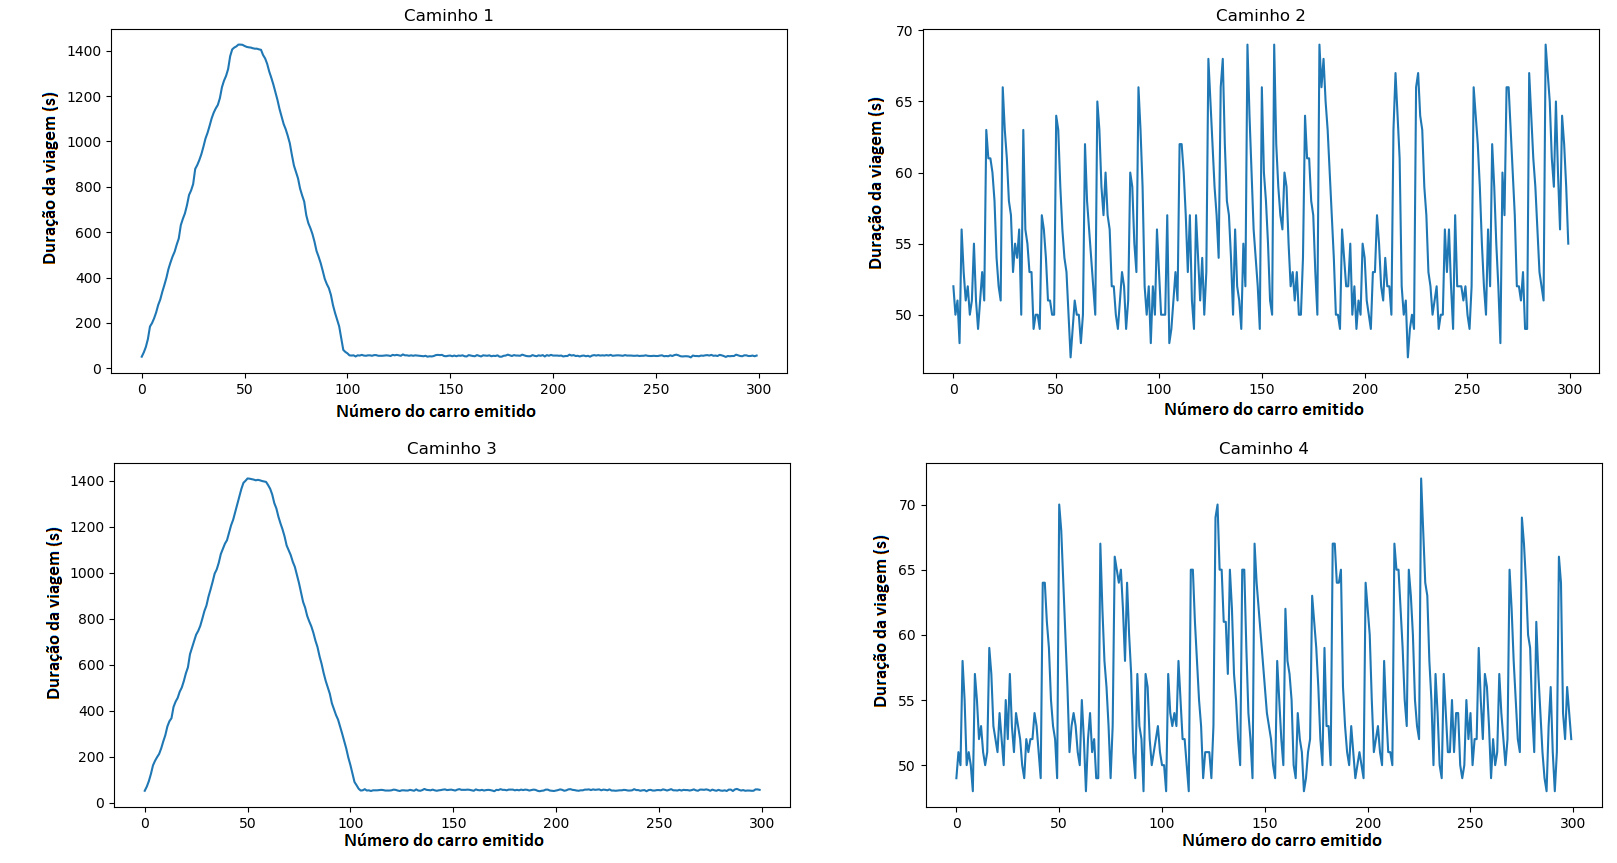
\includegraphics[width=1\textwidth]{figuras/Trip_Duration_No_TrafficLight.PNG}
    \end{center}
    \caption[Duração da viagem, cenário 1]{Simulação sem o sistema.}
    \label{tripNoTL}
\end{figure}

\begin{figure}[H]
    \begin{center}
    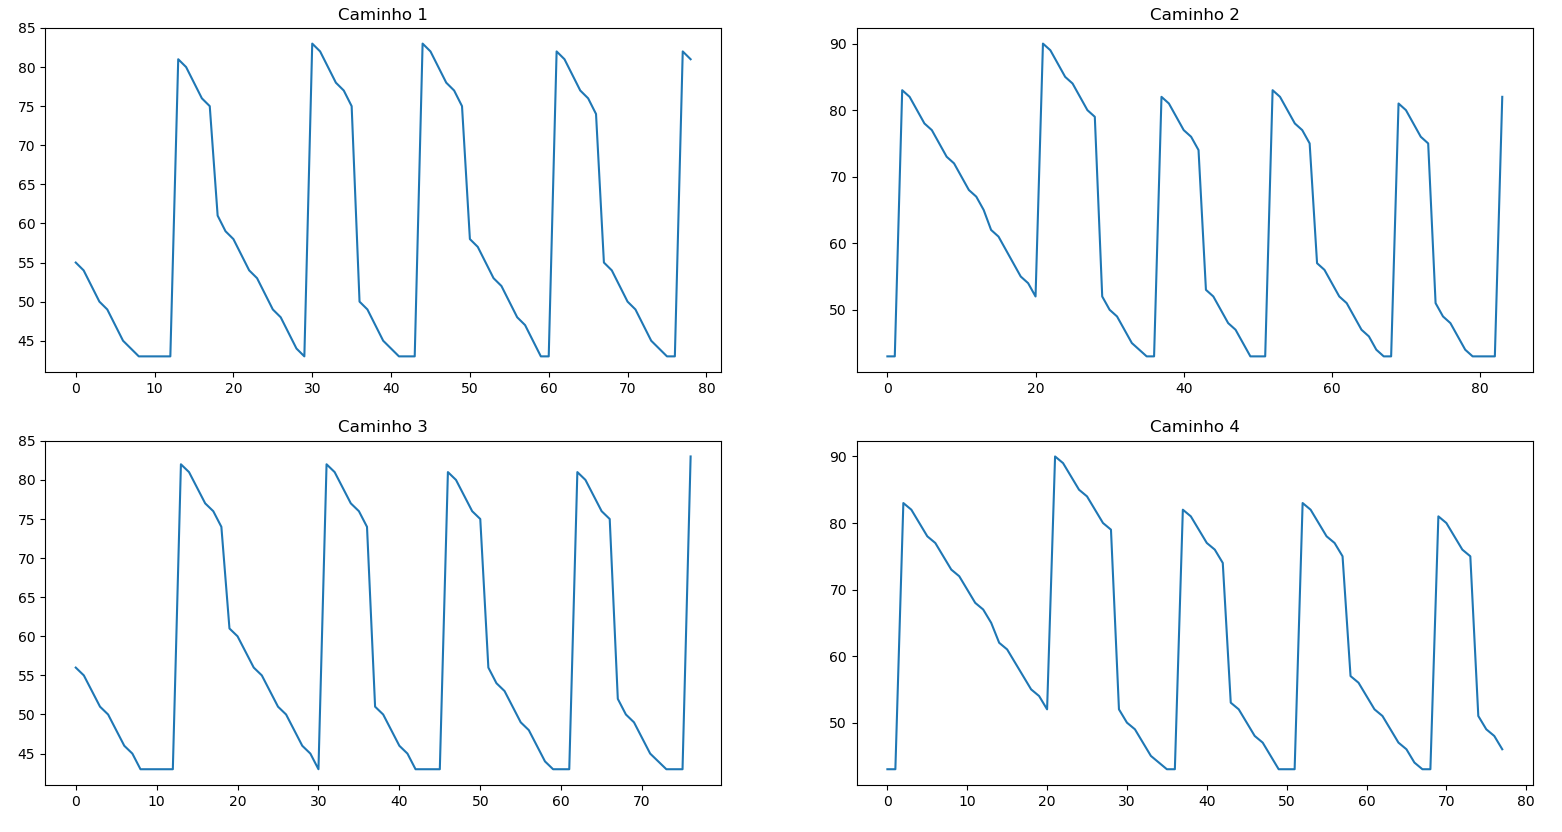
\includegraphics[width=1\textwidth]{figuras/Trip_Duration_With_TrafficLight.PNG}
    \end{center}
    \caption[Duração da viagem, cenário 2]{Simulação com o sistema funcionando com tempos fixos.}
    \label{tripWithTL}
\end{figure}

\begin{figure}[H]
    \begin{center}
    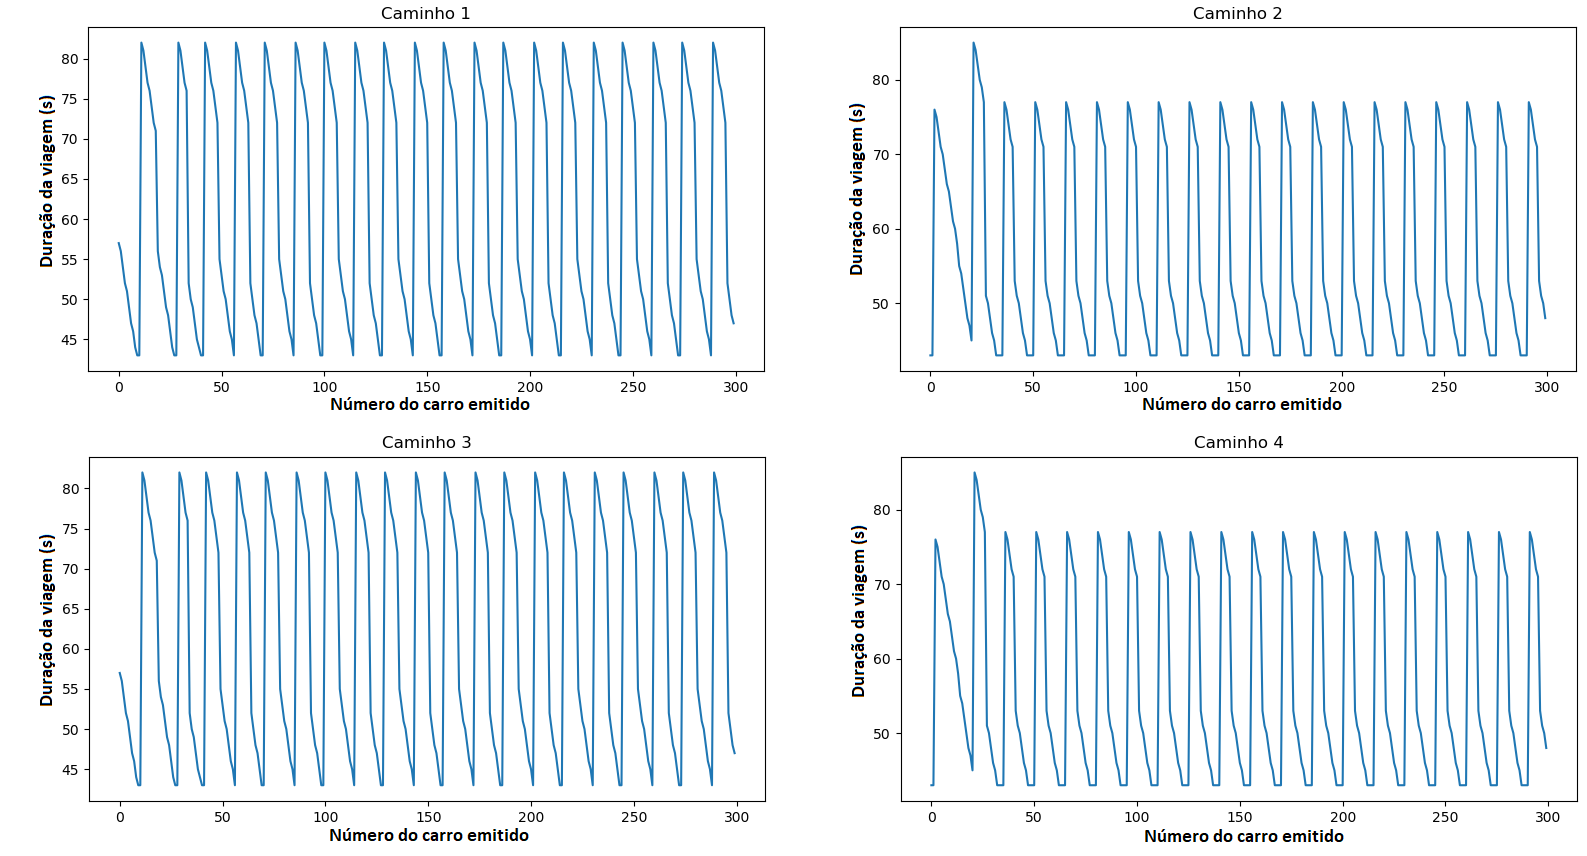
\includegraphics[width=1\textwidth]{figuras/Trip_Duration_With_One_Loop.PNG}
    \end{center}
    \caption[Duração da viagem, cenário 3]{Simulação com o sistema adaptativo com um laço.}
    \label{tripOneLoop}
\end{figure}

\begin{figure}[H]
    \begin{center}
    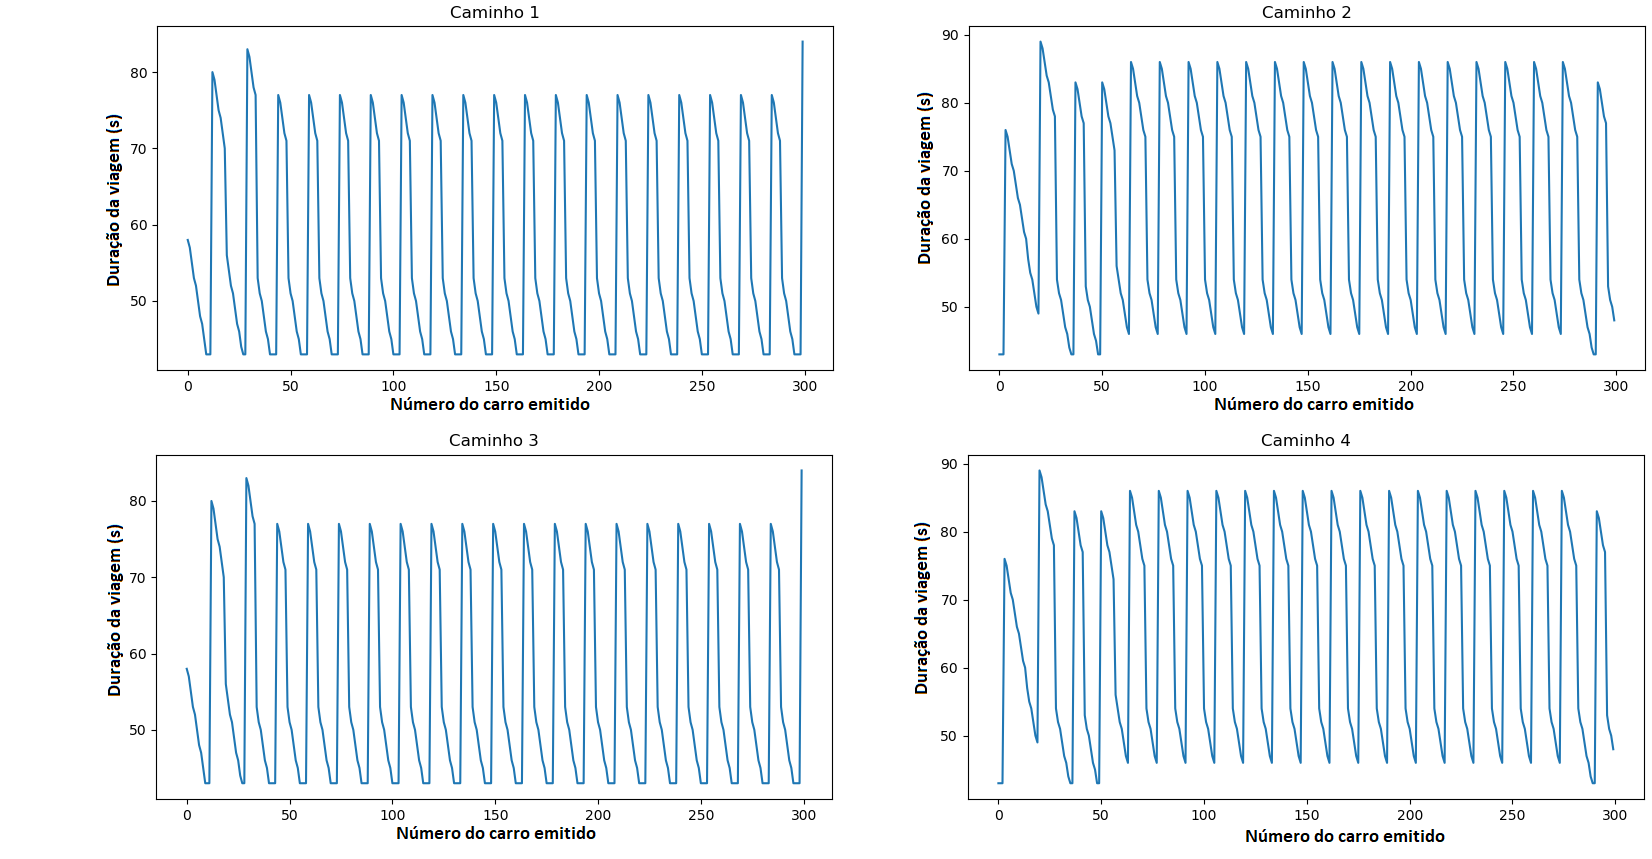
\includegraphics[width=1\textwidth]{figuras/Trip_Duration_With_Two_Loop.PNG}
    \end{center}
    \caption[Duração da viagem, cenário 4]{Simulação com o sistema adaptativo com dois laços.}
    \label{tripTwoLoop}
\end{figure}

Os gráficos gerados confirmam a análise feita com os dados da tabela. É possível observar, no primeiro cenário (simulação sem o sistema), que os gráficos apresentam um comportamento bastante diferente, quando comparados com os outros cenários, devido à falta de organização apresentada no trânsito sem controlador semafórico presente. Pode-se observar que, nos caminhos 1 e 3, a duração da viagem alcançou um valor máximo de 1400 segundos, enquanto os outros caminhos apresentaram um valor máximo de apenas 70 segundos. Esse comportamento representa que os caminhos 2 e 4 "dominaram" o cruzamento, dificultando a passagem dos veículos nos caminhos 1 e 3.

Já nos gráficos das Figuras \ref{tripWithTL}, \ref{tripOneLoop} e \ref{tripTwoLoop}, é possível observar um padrão no comportamento em todos os caminhos. Esse padrão representa o período de abertura de cada semáforo, onde os picos representam os carros que tiveram que esperar o tempo completo de um sinal vermelho, enquanto os vales representam os carros que não precisaram parar em momento algum.
Os valores máximos e mínimos de cada cenário, em cada simulação, podem ser visualizados na Tabela \ref{tab: durationMinMax}.

\begin{table}[H]
\centering
\caption{Valores máximos e mínimos da duração da viagem, em segundos}
\label{tab: durationMinMax}
\begin{tabular}{@{}lllll@{}}
\toprule
Cenário & Caminho 1 & Caminho 2 & Caminho 3 & Caminho 4 \\ \midrule
1 & 1400 / 70 & 70 / 45 & 1400 / 70 & 70 / 45 \\
2 & 80 / 40 & 90 / 40 & 80 / 40 & 90 / 40 \\
3 &	80 / 40 & 85 / 40 & 80 / 40 & 85 / 40 \\
4 & 80 / 40 & 90 / 40 & 80 / 40 & 90 / 40 \\
\bottomrule
\end{tabular}
\end{table}

\section{Tempo de espera em filas}
Seguindo a mesma metodologia de obtenção dos dados referentes à duração das viagens, foram coletados dados referentes ao tempo esperado em filas, para cada caminho. Esse dado é calculado, a cada passo da simulação, medindo a distância entre o ponto de referência (em todos os casos, esse ponto foi o \textit{node} 0 da simulação, ou seja, o cruzamento em si) e o último carro parado no caminho determinado. Diferente da duração de viagem, o tempo de espera em filas é gerado a cada passo da simulação, representando 1 segundo. Esse parâmetro não é calculado para cada veículo, mas para o conjunto de veículos que se encontra em um determinado caminho.

Novamente, com os dados obtidos a partir da simulação, foi possível construir a Tabela \ref{tab: queue} com os valores das médias do parâmetro, assim como traçar um gráfico para cada caminho, em cada cenário.

\begin{table}[H]
\centering
\caption{Tempo médio de espera em filas, e o respectivo desvio padrão, em segundos}
\label{tab: queue}
\begin{tabular}{@{}llllll@{}}
\toprule
Cenário & Caminho 1 & Caminho 2 & Caminho 3 & Caminho 4 & Total \\ \midrule
1 & 222 $\pm$ 50 & 172 $\pm$ 112 & 220 $\pm$ 52 & 173 $\pm$ 112 & 197 $\pm$ 81 \\
2 & 21 $\pm$ 10 & 23 $\pm$ 13 & 21 $\pm$ 10 & 23 $\pm$ 13 & 22 $\pm$ 12 \\
3 &	23 $\pm$ 11 & 18 $\pm$ 9 & 23 $\pm$ 11 & 18 $\pm$ 9 & 21 $\pm$ 10 \\
4 & 17 $\pm$ 8 & 26 $\pm$ 12 & 17 $\pm$ 8 & 26 $\pm$ 12 & 21 $\pm$ 10 \\
\bottomrule
\end{tabular}
\end{table}

Observando a Tabela \ref{tab: queue}, nota-se um comportamento semelhante ao da Tabela \ref{tab: duration}, onde os resultados obtidos no primeiro cenário apresentam valores destoantes com os outros cenários. Isso se deve, como foi analisado anteriormente, pela falta de um elemento para organizar os fluxos veiculares no cruzamento. Nos cenários 2, 3 e 4, existe uma redução no tempo de espera em todos os caminhos, demonstrando uma melhoria, nos cenários em que o sistema estava instalado. Quando comparamos as Tabelas \ref{tab: duration} e \ref{tab: queue}, pode-se observar uma coerência no comportamento dos valores de cada cenário, demonstrando o impacto do sistema nos dois parâmetros observados.

Os gráficos das Figuras \ref{queueNoTL} a \ref{queueTwoLoop}  apresentam os dados referentes ao tempo de espera em filas, das quatro simulações.O eixo vertical de cada gráfico representa o tempo, em segundos, das filas formadas em cada caminho. O eixo horizontal representa o tempo de simulação, em segundos. Cada segundo representa um passo da simulação.

Esses dados são calculados pela simulação, e disponibilizados nos arquivos de \textit{output}. A cada passo da simulação, é calculada a duração, em segundos, das filas formadas em cada caminho. O tempo em filas é calculado pelo tempo que os veículos ficam parados na via.

\begin{figure}[H]
    \begin{center}
    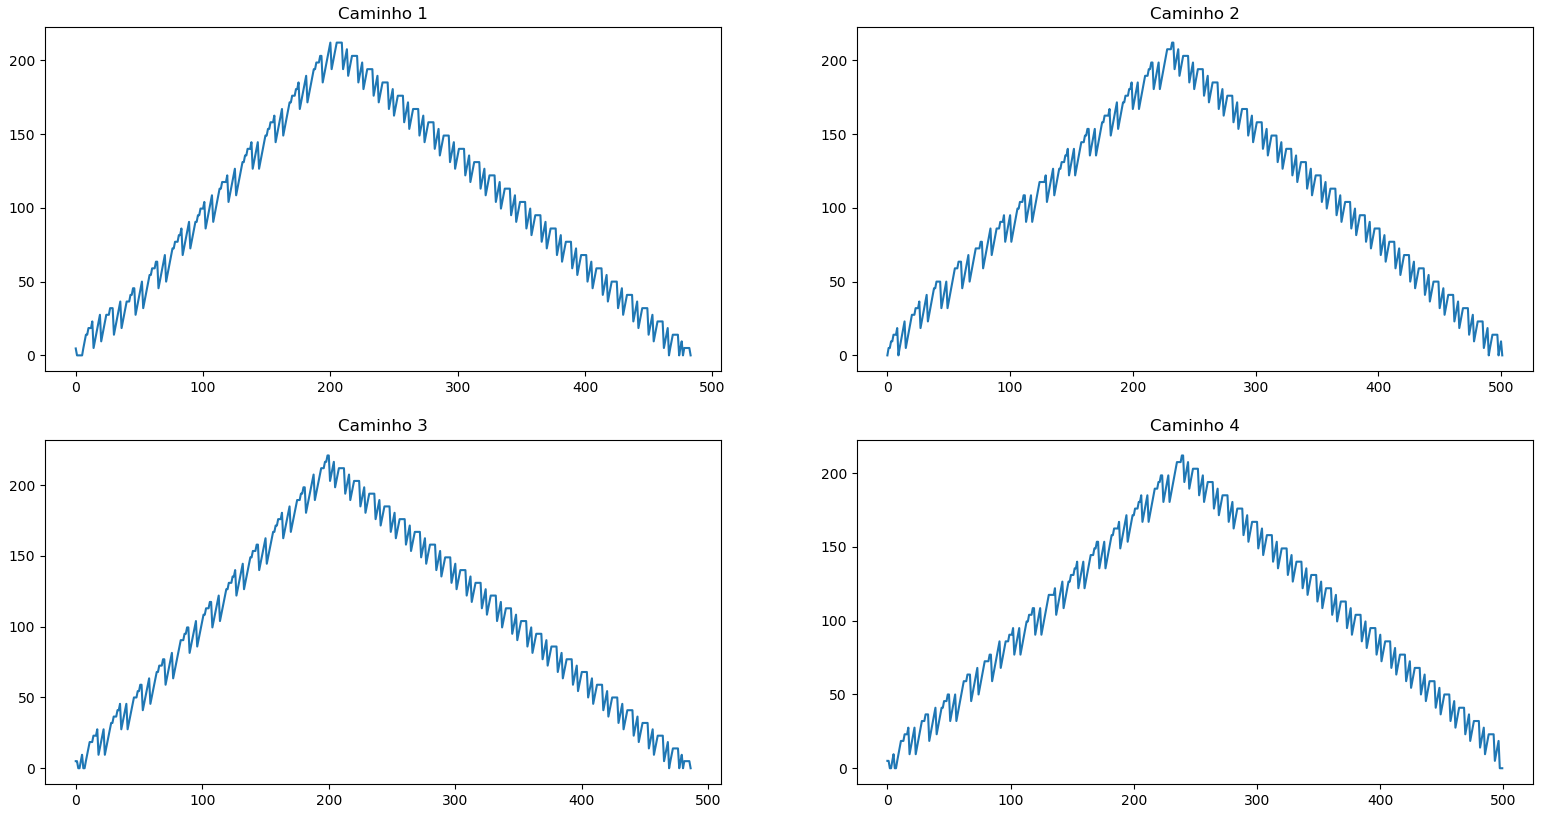
\includegraphics[width=0.8\textwidth]{figuras/Queue_Duration_No_TrafficLight.PNG}
    \end{center}
    \caption[Duração das filas, cenário 1]{Simulação sem o sistema.}
    \label{queueNoTL}
\end{figure}

\begin{figure}[H]
    \begin{center}
    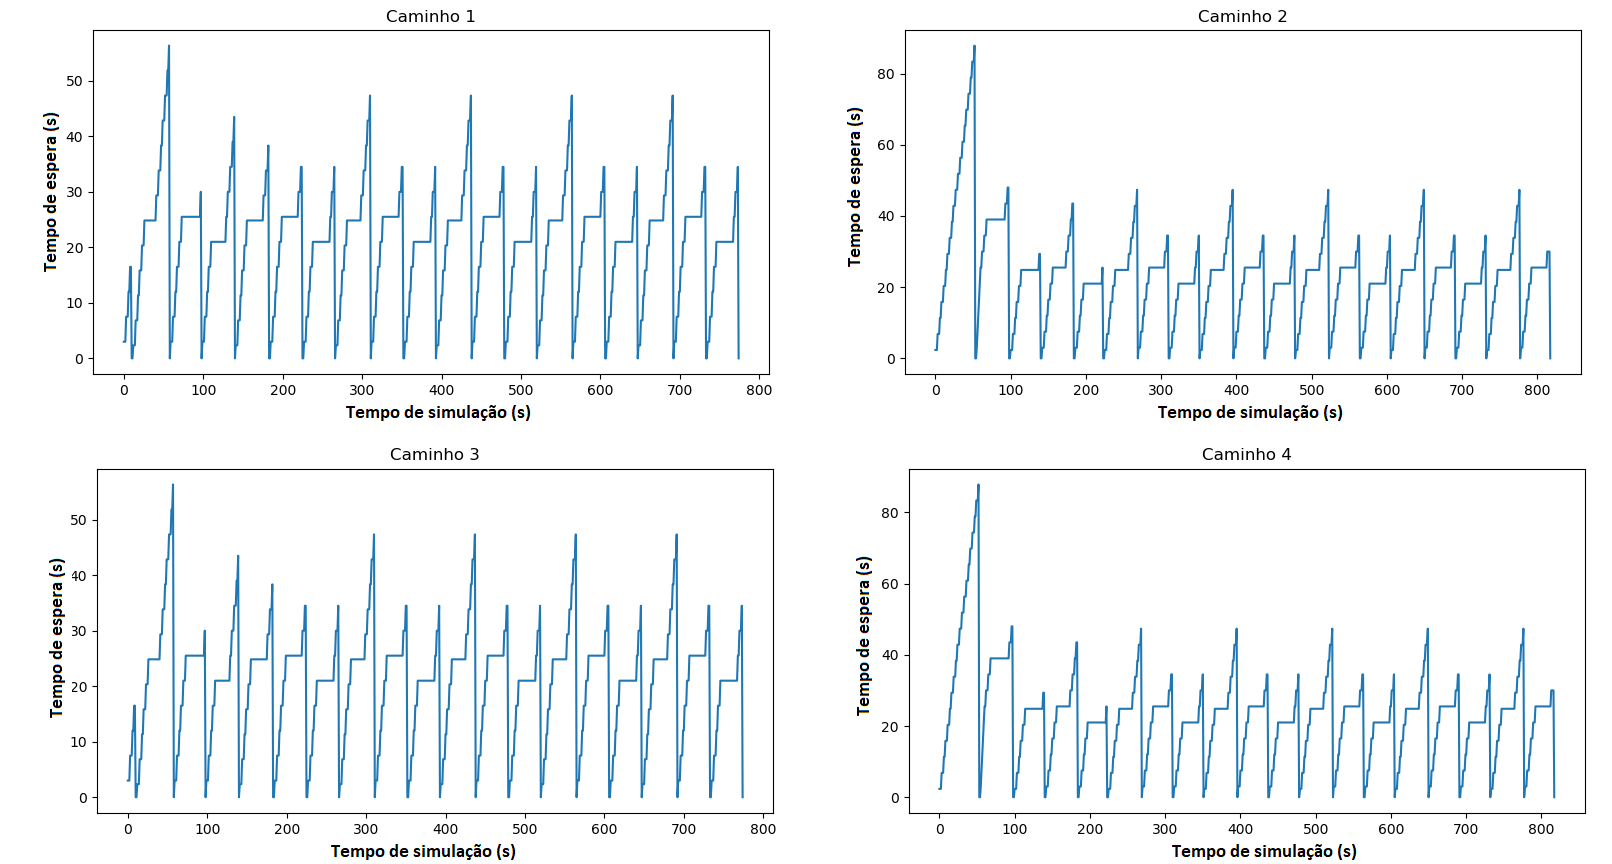
\includegraphics[width=0.8\textwidth]{figuras/Queue_Duration_With_TrafficLight.PNG}
    \end{center}
    \caption[Duração das filas, cenário 2]{Simulação com o sistema funcionando com tempos fixos.}
    \label{queueWithTL}
\end{figure}

\begin{figure}[H]
    \begin{center}
    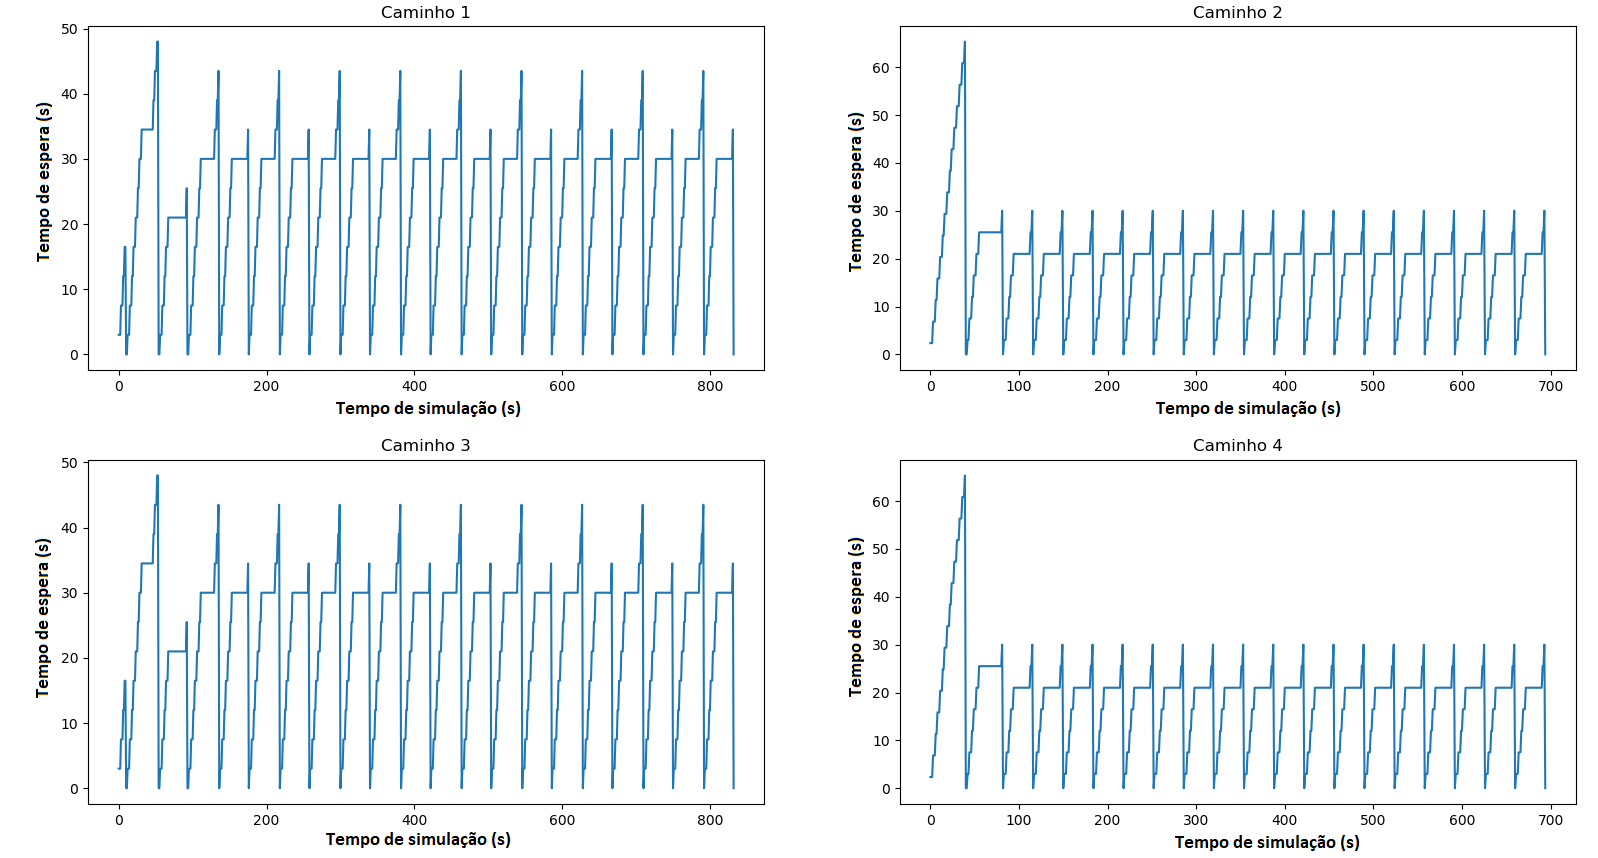
\includegraphics[width=0.8\textwidth]{figuras/Queue_Duration_With_One_Loop.PNG}
    \end{center}
    \caption[Duração das filas, cenário 3]{Simulação com o sistema adaptativo com um laço.}
    \label{queueOneLoop}
\end{figure}

\begin{figure}[H]
    \begin{center}
    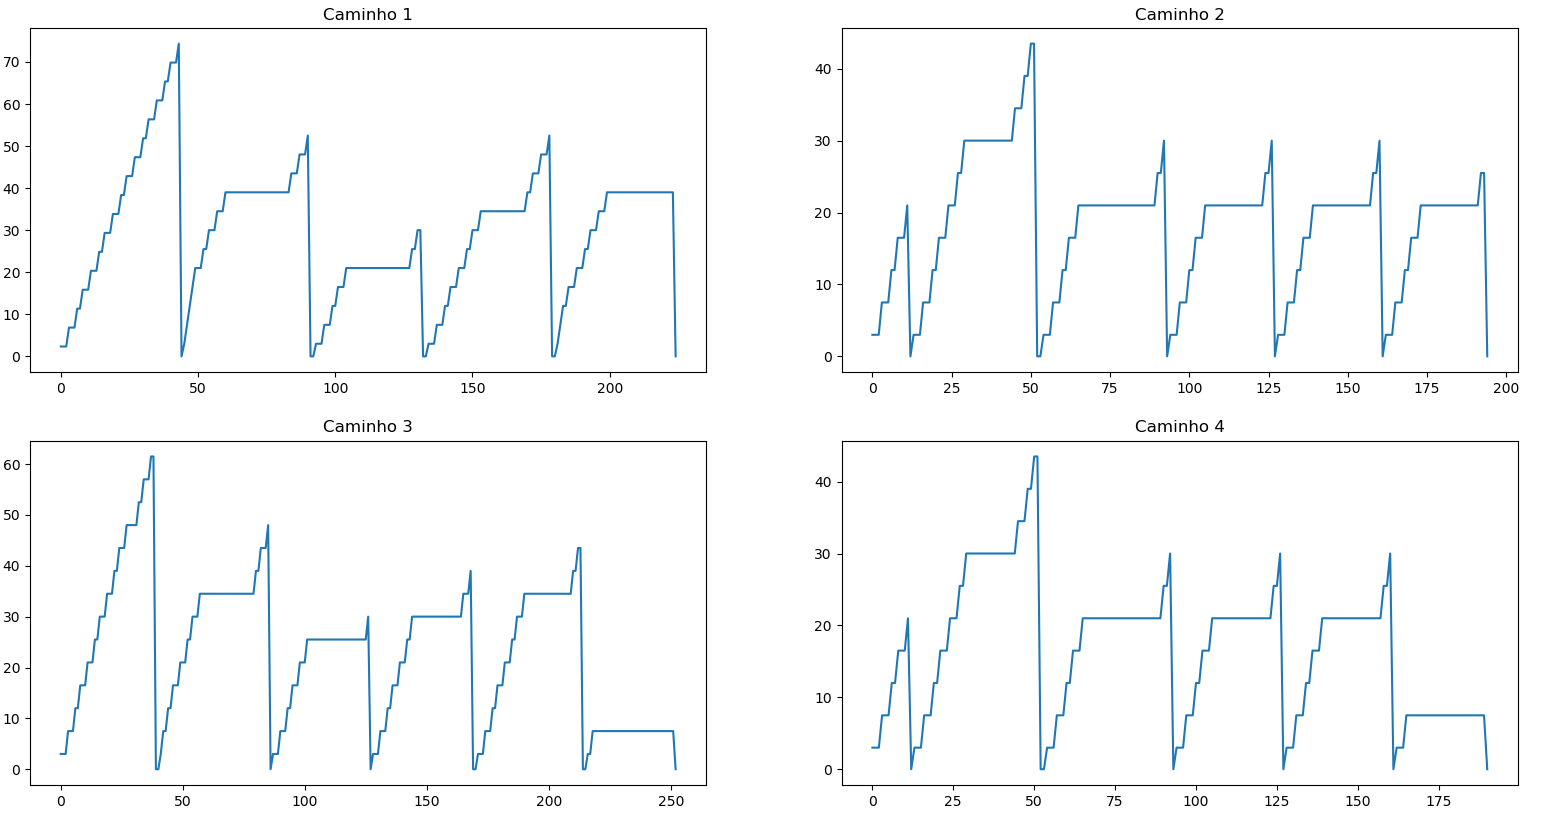
\includegraphics[width=0.8\textwidth]{figuras/Queue_Duration_With_Two_Loop.PNG}
    \end{center}
    \caption[Duração das filas, cenário 4]{Simulação com o sistema adaptativo com dois laços.}
    \label{queueTwoLoop}
\end{figure}

O comportamento dos gráficos gerados apresentam uma coerência com os valores observados na Tabela \ref{tab: queue}. No primeiro cenário, os gráficos apresentam um comportamento bastante diferente dos apresentados nos outros cenários, por conta da falta de organização dos fluxos veiculares. Por conta da falta de um elemento que organize o trânsito, os gráficos apresentam um comportamento imprevisível, sem um padrão de repetição, que é observado nos cenários que possuem o semáforo funcionando.

Assim como foi observado na sessão anterior, os gráficos das Figuras \ref{queueWithTL}, \ref{queueOneLoop} e \ref{queueTwoLoop} apresentam um padrão no comportamento em todos os caminhos, condizente com o período de abertura de cada semáforo. Os valores máximos e mínimos de cada cenário, em cada simulação, podem ser visualizados na Tabela \ref{tab: queueMinMax}.

\begin{table}[H]
\centering
\caption{Valores máximos e mínimos do tempo de espera em filas, em segundos}
\label{tab: queueMinMax}
\begin{tabular}{@{}lllll@{}}
\toprule
Cenário & Caminho 1 & Caminho 2 & Caminho 3 & Caminho 4 \\ \midrule
1 & 250 / 0 & 250 / 0 & 250 / 0 & 250 / 0 \\
2 & 50 / 0 & 60 / 0 & 50 / 0 & 60 / 0 \\
3 &	50 / 0 & 60 / 0 & 50 / 0 & 60 / 0 \\
4 & 40 / 0 & 60 / 0 & 40 / 0 & 60 / 0 \\
\bottomrule
\end{tabular}
\end{table}

\section{Desempenho do sistema}

Ao observar os valores das tabelas, percebe-se que a implementação do sistema teve um impacto bastante positivo no fluxo de veículos. No caso da duração da viagem, houve uma redução de até $68,54\%$, se comparados os valores das médias do caminho 4 para os cenários 1 e 4. Já no caso do tempo de espera em filas apresentou uma redução de até $83,81\%$, comparando os valores das médias do caminho 4, para os cenários 1 e 2 (essa mesma melhoria foi observada em outros cenários). Ainda se forem observados os piores casos, há uma redução de $62,57\%$ no tempo de viagens, e $71,57\%$ no tempo de espera nas filas, levando em conta os valores médios.

Observando os gráficos, é fácil reconhecer, tanto na duração da viagem, quanto no tempo de filas, que há um padrão no comportamento do fluxo veicular, quando o sistema está em funcionamento. Percebe-se isso comparando os gráficos dos cenários 2, 3 e 4, onde os picos representam momentos de semáforo fechado, e os vales representam os momentos de semáforo aberto.. 

No caso da duração das viagens, nota-se, nos gráficos do primeiro cenário, que esse parâmetro atinge o pico nos primeiros 50 carros da simulação, nos caminhos 1 e 3, chegando ao valor de 1400 segundos de duração. Após esse pico, existe uma redução e, por fim, estabilidade do parâmetro, quando os veículos conseguem fluir, sem trânsito.
Já nos caminhos 2 e 4, pode-se observar que os tempos de viagem se mantêm em um intervalo mais controlado, com menor variação, apesar de não apresentar um padrão.

Nos cenários 2, 3 e 4, porém, nota-se que os gráficos apresentam comportamentos semelhantes entre si, em que o tempo de viagem sofre um leve aumento, durante o período de semáforo fechado, mas volta a cair quando ocorre a abertura. Nenhum caminho, de nenhum cenário, apresentou duração de viagem superior a 100 s, demonstrando a eficácia do sistema. 
Quando comparamos os piores casos (valores máximos) observados em cada simulação, na Tabela \ref{tab: durationMinMax}, notamos uma melhoria de até $94,3\%$ no tempo de viagem, comparando os piores valores do caminho 1 no primeiro e segundo cenários.

No caso do tempo de espera em filas, o primeiro ponto a ser notado é que, no primeiro cenário, os gráficos dos caminhos 1 e 3 apresentam muito mais valores de tempo de simulação. Isso é devido à formação de trânsito, fazendo com que os veículos precisem de mais tempo para completar o percurso, com isso, o tempo necessário para completar a simulação dos caminhos 1 e 3 é $95\%$ maior que o necessário para os caminhos 2 e 4.
Nos cenários 2, 3 e 4, observa-se um comportamento semelhante aos gráficos de duração da viagem, onde o parâmetro sofre um aumento durante o tempo de semáforo fechado, seguido por uma melhora, quando o fluxo é liberado.
Nesses casos, quando comparamos os piores casos dos tempos de espera em filas, na Tabela \ref{tab: queueMinMax}, notamos uma redução de até $84\%$, quando usamos os piores valores do caminho 1, no primeiro e quarto cenários.

Com esses resultados, é possível notar que existe uma correlação entre os dois parâmetros observados. Âmbos apresentaram uma melhoria significativa com a implementação do sistema. A duração do percurso é limitada pelo tempo de abertura do semáforo, enquanto o tempo em filas (efetivamente o tempo que o veículo passa parado) é limitado pelo tempo em que o semáforo permanece fechado.

Uma observação a ser feita, é que não houve melhoria no sistema, ao aumentar a quantidade de detectores utilizados. Isso se deve pela simplicidade do cenário, pois o detector é utilizado para trocar a prioridade da via, e com apenas duas fases do semáforo, apenas um detector é suficiente para realizar o controle semafórico. Outro fato, que poderia justificar o uso do sistema adaptativo com o uso de sensores, seria a emissão de veículos. Nos cenários apresentados, o fluxo veicular foi constante e idêntico em todos os caminhos, portanto, aumentar a prioridade para um determinado fluxo acarretaria em uma piora para os demais fluxos.